\documentclass[10pt]{article}

\usepackage{mathtools}  % need for math tools
\usepackage{amsmath}    % need for subequations
\usepackage{graphicx}   % need for figures
\usepackage{verbatim}   % useful for program listings
\usepackage{color}      % use if color is used in text
\usepackage{subfigure}  % use for side-by-side figures
\usepackage{hyperref}   % use for hypertext links, including those to external documents and URLs
\usepackage{graphicx}   % Used to import the graphics

\setlength{\baselineskip}{16.0pt}   
\setlength{\parskip}{3pt plus 2pt}
\setlength{\parindent}{20pt}
\setlength{\oddsidemargin}{0.5cm}
\setlength{\evensidemargin}{0.5cm}
\setlength{\marginparsep}{0.75cm}
\setlength{\marginparwidth}{2.5cm}
\setlength{\marginparpush}{1.0cm}
\setlength{\textwidth}{150mm}



\begin{document}

\begin{center}
{\large Ay190: Computational Astrophysics (Winter Term 2012)} \\
{\large HomeWork - 3 } \\
\copyright 2012 by Arya Farahi \\
Jan 16, 2012
\end{center}

\section{Exercise 1. Integration via Newton-Cotes Formulae}

\begin{figure}[hbt]
  \begin{center}
    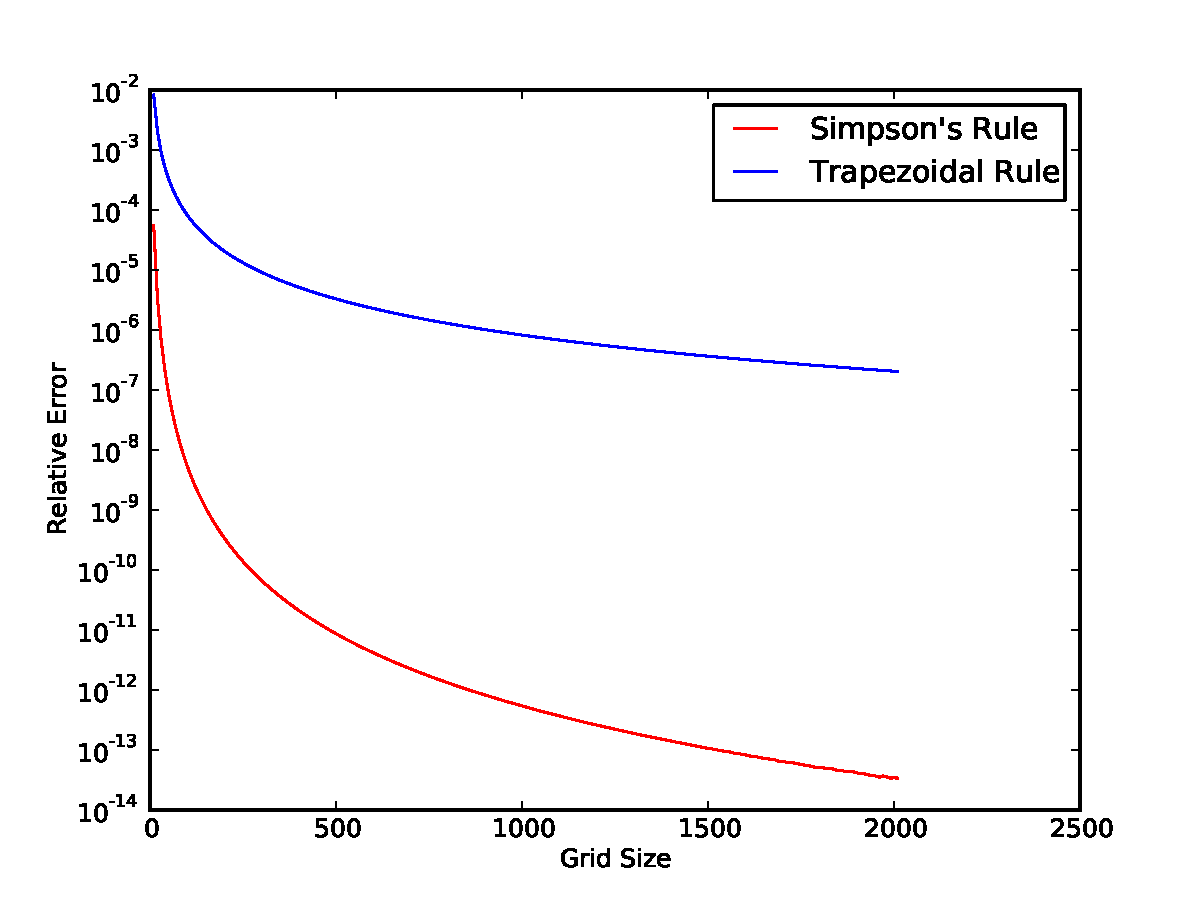
\includegraphics[scale=0.7]{Plot/plot1.pdf}
    \caption{\label{fig:RelErr} Plot of the relative error for Intgral of $ f(x)=x sin(x) $ with Simpson's Rule and Trapezoidal Rule in semilogaritmic scale.}
  \end{center}
\end{figure}

Figure \ref{fig:RelErr} showes plot of the relative error for Intgral of $ f(x)=x sin(x) $ with Simpson's Rule and Trapezoidal Rule in semilogaritmic scale. It is obvious that for both method the numerical method converge to real answer but the convergence rate for Simpson's rule is faster than the other one. In this plot our grid size starts from 10 point to 2000 point in the integeral range. \\

\section{Exercise 2. Gaussian Quadrature}

 The density of electrons in this environment by useing Gauss-Laguerre Quadrature and Trapezoidal Rule method for finding the numerical integral is same and it is equal to : $1.90216 \times 10^{41}$. We used 50 pionts for finding the answer of integral.\\

In the second part we want to use Gaussian-Legendre Quadrature for each specific $ \Delta E $ and finding the whole integral by simply adding the answer of each part. So we have the following equations:  

\begin{equation}\label{eq:eq1}
 n_{e^{\pm}} = \frac{8 \pi}{(2 \pi \hbar)^3 } \int_0^\infty \frac{p^2 dp}{e^{\beta cp}+1} = \frac{8 \pi}{(2 \pi \hbar c)^3 } \int_0^\infty \frac{(cp)^2 d(cp)}{e^{\beta cp}+1} 
\end{equation}

If $E = cp$ then we have: \\

\begin{equation}\label{eq:eq2}
 n_{e^{\pm}} = \frac{8 \pi}{(2 \pi \hbar c)^3 } \int_0^\infty \frac{E^2 dE}{e^{\beta E}+1} 
\end{equation}

Then: \\

\begin{equation}\label{eq:eq3}
 n_{e^{\pm}} = \frac{8 \pi}{(2 \pi \hbar c)^3 } \int_0^\infty \frac{E^2 dE}{e^{\beta E}+1} = \frac{8 \pi}{(2 \pi \hbar c)^3 } \sum \int_{E_i}^{E_i + \Delta E} \frac{E^2 dE}{e^{\beta E}+1}
\end{equation}

For each $\delta E$ range we calculate the integral by Gaussian-Legendre Quadrature method. We used 10 points for finding the integral by Gaussian-Legendre Quadrature method. And we choose $\Delta E = 3 MeV$ and $E_{max} = 450 MeV$ because for $E$ more than $450 MeV$ the integral is negligible. And the final answer is the same as the answer of equation \ref{eq:eq1}. \\

Figure \ref{fig:SpeDis} shows the spectral distribution of density of electrons in this environment. It is obvoius that after $450 Mev$ it is negiligble and we can ignore that for calculating the integral.\\

\begin{figure}[hbt]
  \begin{center}
    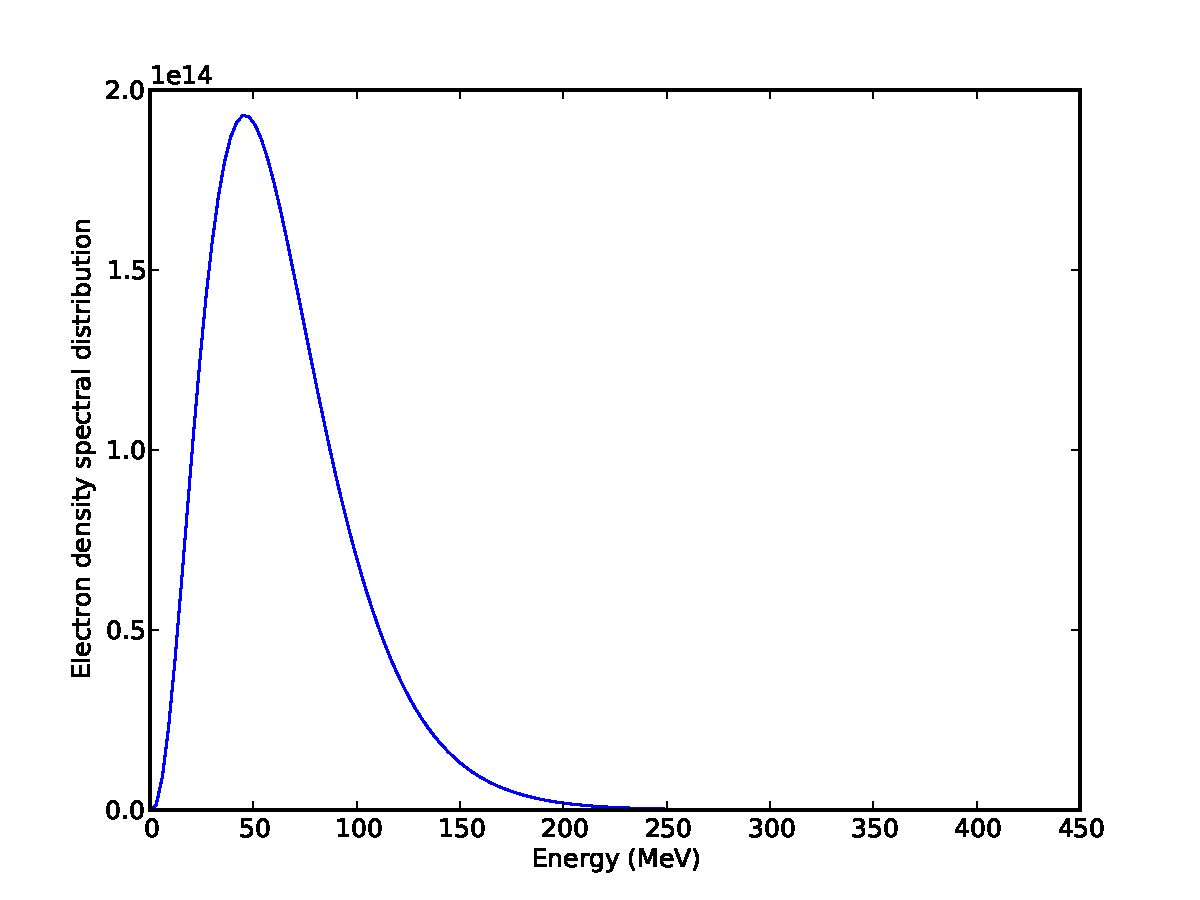
\includegraphics[scale=0.7]{Plot/plot2.pdf}
    \caption{\label{fig:SpeDis} Plot of density of electrons's spectral distribution.}
  \end{center}
\end{figure}


\end{document}
